% =======================================================================================================
\section{Metodologia experimental}
\label{sec:metodo}

Um resultado sem protocolo não é um resultado: é uma coincidência documentada. Esta seção descreve
como o modelo foi avaliado, por que cada escolha foi feita e quais são suas limitações. O objetivo
é que qualquer leitor possa repetir a análise e obter os mesmos números.

\subsection{Visão geral}

O protocolo tem cinco etapas:

\begin{enumerate}
	\item \textbf{separação}: divisão estratificada em treino (70\,\%) e teste (30\,\%), com o teste
	      reservado e usado uma única vez;
	\item \textbf{seleção}: comparação de arquiteturas, ativações e regularização por validação
	      cruzada \emph{apenas no treino};
	\item \textbf{treinamento final}: ajuste do modelo escolhido em todo o conjunto de treino;
	\item \textbf{avaliação}: uma única medida no conjunto de teste, com intervalo de confiança;
	\item \textbf{comparação}: repetição do procedimento para modelos alternativos, com as mesmas
	      dobras, e teste estatístico pareado.
\end{enumerate}

A separação entre \emph{seleção} e \emph{avaliação final} é o ponto mais importante. Se o mesmo
conjunto serve para escolher hiperparâmetros e para reportar desempenho, o resultado fica otimista:
o modelo foi escolhido, entre muitas opções, justamente por ter ido bem naquele conjunto. A
validação cruzada dentro do treino resolve a seleção; o teste, intocado, fornece a estimativa
honesta.

\subsection{Divisão treino/teste}

A divisão usa amostragem \emph{estratificada}: a proporção de cada classe é preservada nos dois
subconjuntos. Com 150 amostras e 30\,\% para teste, cada classe contribui com 15 amostras no teste
e 35 no treino, totalizando \nTeste{} e \nTreino{} amostras, respectivamente. A semente é fixa
(\texttt{random\_state=42}), de modo que a divisão é sempre a mesma.

\begin{figure}[htbp]
	\centering
	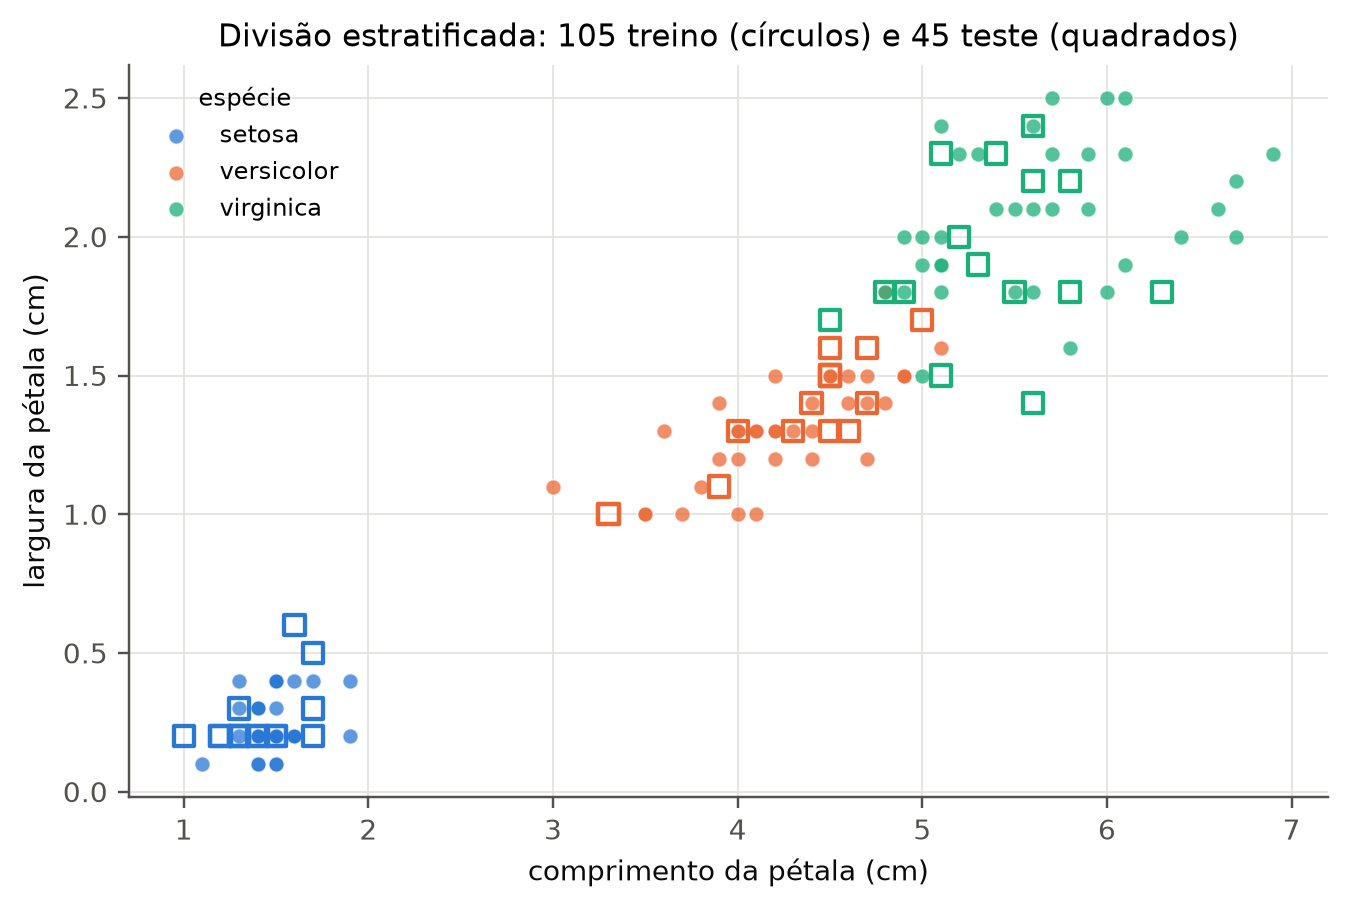
\includegraphics[width=0.72\textwidth]{fig_divisao_treino_teste.png}
	\caption{Divisão estratificada no plano das duas variáveis mais informativas. Círculos são
	amostras de treino (\nTreino{}) e quadrados vazados são amostras de teste (\nTeste{}). A
	proporção de cada espécie é preservada nos dois subconjuntos.}
	\label{fig:divisao}
\end{figure}

\paragraph{Por que estratificar.} Com 150 amostras, uma divisão puramente aleatória pode deixar
uma classe sub-representada no teste, o que aumenta a variância da estimativa. A estratificação
garante que o teste reflita a composição do problema.

\paragraph{Por que não usar o teste para nada além da medida final.} Cada vez que se olha o teste
e se toma uma decisão com base nele, ele deixa de ser um teste. Ajustar hiperparâmetros,
escolher a semente ou descartar um resultado ``estranho'' com base no teste contamina a
estimativa \cite{kaufman2012}.

\subsection{Validação cruzada}

A validação cruzada $k$-fold divide o conjunto de treino em $k$ partes iguais e, em cada rodada,
usa uma parte para validação e as outras $k-1$ para ajuste. Ao final, cada amostra foi usada
exatamente uma vez para validação. O estimador é a média das $k$ medidas:

\begin{equation}
	\widehat{\text{acc}}_{\text{CV}} = \frac{1}{k}\sum_{j=1}^{k} \text{acc}_j,
	\qquad
	\widehat{\text{se}} = \frac{s}{\sqrt{k}},
	\quad s^2 = \frac{1}{k-1}\sum_{j=1}^{k}\left(\text{acc}_j - \widehat{\text{acc}}_{\text{CV}}\right)^2.
	\label{eq:cv}
\end{equation}

Neste trabalho usa-se $k=5$ com estratificação, repetido $R=5$ vezes com sementes diferentes,
totalizando 25 medidas. A repetição reduz a dependência de uma partição específica
\cite{kohavi1995}. O desvio-padrão reportado é o das 25 dobras, não o erro-padrão da média: ele
mede a variabilidade entre partições, que é o que interessa para comparar configurações.

A \figura{fig:kfold} ilustra o esquema com $k=5$: em cada linha, o bloco destacado é a dobra de
validação e os demais são de treino.

\begin{figure}[htbp]
	\centering
	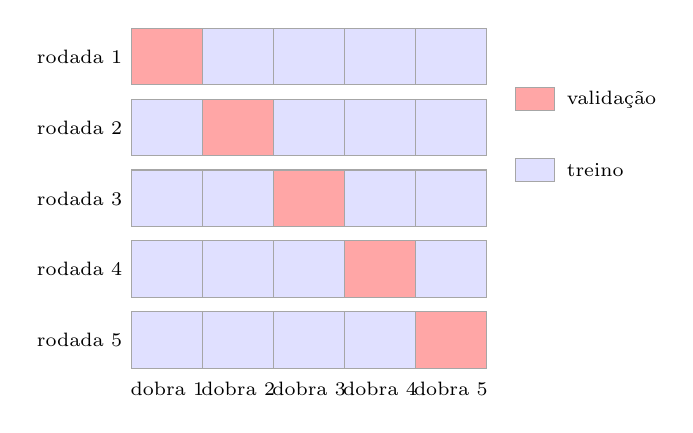
\begin{tikzpicture}[font=\scriptsize,x=0.9cm,y=0.9cm]
		\foreach \r in {1,...,5}{
			\foreach \c in {1,...,5}{
				\pgfmathtruncatemacro{\teste}{\r==\c}
				\ifnum\teste=1
					\fill[red!35] (\c-1,-\r) rectangle ++(1,0.8);
				\else
					\fill[blue!12] (\c-1,-\r) rectangle ++(1,0.8);
				\fi
				\draw[gray!70] (\c-1,-\r) rectangle ++(1,0.8);
			}
			\node[left] at (0,-\r+0.4) {rodada \r};
		}
		\foreach \c in {1,...,5}{
			\node[below] at (\c-0.5,-5.05) {dobra \c};
		}
		\node[anchor=west,fill=red!35,draw=gray!70,minimum width=0.5cm,minimum height=0.3cm] at (5.4,-1.2) {};
		\node[anchor=west] at (6.0,-1.2) {validação};
		\node[anchor=west,fill=blue!12,draw=gray!70,minimum width=0.5cm,minimum height=0.3cm] at (5.4,-2.2) {};
		\node[anchor=west] at (6.0,-2.2) {treino};
	\end{tikzpicture}
	\caption{Esquema da validação cruzada $k$-fold com $k=5$. Cada amostra é usada uma vez para
	validação e quatro vezes para treino. A estimativa final é a média das cinco rodadas.}
	\label{fig:kfold}
\end{figure}

\paragraph{Vazamento de informação.} O pré-processamento faz parte do modelo e deve ser ajustado
dentro de cada dobra. Por isso o código usa um \texttt{Pipeline}: a padronização é ajustada apenas
nas amostras de treino da dobra e aplicada às de validação. Se a padronização fosse ajustada no
conjunto completo, a média e o desvio conteriam informação do conjunto de validação --- vazamento
sutil, mas real \cite{kaufman2012}.

\subsection{Seleção de hiperparâmetros}

As varreduras usam 3 repetições de 5 dobras (15 ajustes por configuração), o que mantém o custo
baixo e já é suficiente para revelar tendências. O modelo final é escolhido pelos resultados
dessas varreduras e reavaliado no teste:

\begin{itemize}
	\item \textbf{arquitetura}: nove configurações, de $(4)$ a $(128,64)$, e a contagem de
	      parâmetros correspondente;
	\item \textbf{ativação}: ReLU, \emph{tanh}, logística e identidade, com a mesma arquitetura
	      $(16,8)$;
	\item \textbf{regularização}: $\alpha \in \{10^{-6},\dots,10^{2}\}$, em escala logarítmica, com
	      a arquitetura $(32,16)$;
	\item \textbf{taxa de aprendizado}: SGD com momento, taxas de $10^{-3}$ a $5\times10^{-1}$.
\end{itemize}

A configuração adotada --- uma camada oculta com 16 neurônios, ativação \emph{tanh} e
$\alpha = 10^{-2}$ --- é uma escolha de compromisso entre as três varreduras: a \emph{tanh} foi a
ativação com melhor acurácia, $\alpha = 10^{-2}$ está no centro da faixa estável e 16 neurônios é
uma capacidade intermediária, nem mínima nem excessiva. Ela não é o máximo absoluto de nenhuma
varredura isolada --- a rede de 4 neurônios teve acurácia ligeiramente maior ---, e essa diferença
está dentro do ruído entre dobras. Como a escolha foi feita sobre os dados de treino, a estimativa
de validação cruzada do modelo final é ligeiramente otimista; o conjunto de teste, mantido à
parte, é a medida que não sofre esse efeito.

\subsection{Métricas de avaliação}
\label{sec:metricas}

Para um problema de classificação, a acurácia isolada esconde informação. As métricas usadas são
definidas a seguir, para uma classe $k$ com verdadeiros positivos $TP_k$, falsos positivos $FP_k$
e falsos negativos $FN_k$.

\begin{align}
	\text{acurácia} &= \frac{1}{n}\sum_{i=1}^{n}\indic\left[\hat{y}_i = y_i\right],
	\label{eq:acc}\\
	\text{precisão}_k &= \frac{TP_k}{TP_k+FP_k}, \qquad
	\text{revocação}_k = \frac{TP_k}{TP_k+FN_k},
	\label{eq:pr}\\
	F_{1,k} &= \frac{2\,\text{precisão}_k\,\text{revocação}_k}{\text{precisão}_k+\text{revocação}_k},
	\label{eq:f1}\\
	F_1^{\text{macro}} &= \frac{1}{C}\sum_{k=1}^{C} F_{1,k}. \label{eq:f1macro}
\end{align}

A precisão responde ``quando o modelo diz classe $k$, ele acerta?''. A revocação responde ``de
tudo que era classe $k$, quanto o modelo encontrou?''. O $F_1$ é a média harmônica das duas e pune
desequilíbrios. A média \emph{macro} dá o mesmo peso a todas as classes, independentemente do
tamanho; é a escolha correta quando as classes importam igualmente --- como aqui.

\paragraph{Entropia cruzada.} Para avaliar a \emph{calibração} das probabilidades, usa-se
\begin{equation}
	\text{LogLoss} = -\frac{1}{n}\sum_{i=1}^{n}\sum_{k=1}^{C} y_{ik}\log p_{ik},
	\label{eq:logloss}
\end{equation}
que penaliza confiança indevida. Um modelo pode ter acurácia alta e LogLoss ruim se acertar com
probabilidade $0{,}51$ em vez de $0{,}95$. Neste relatório, a LogLoss aparece nas varreduras
porque ela distingue configurações que a acurácia considera empatadas.

\paragraph{Matriz de confusão.} A matriz $C_{jk}$ conta quantas amostras da classe $j$ foram
previstas como $k$. Ela mostra \emph{para onde} vão os erros, o que a acurácia não mostra. No
\secao{sec:resultados}, a matriz revela que os erros se concentram na fronteira
\emph{versicolor}--\emph{virginica}.

\subsection{Incerteza das estimativas}

Com $n=45$ amostras de teste, uma acurácia de $93{,}3\,\%$ corresponde a 42 acertos. O intervalo de
confiança de Wilson, adequado para proporções com $n$ pequeno, é
\begin{equation}
	\frac{\hat{p} + \frac{z^2}{2n} \pm z\sqrt{\frac{\hat{p}(1-\hat{p})}{n} + \frac{z^2}{4n^2}}}{1+\frac{z^2}{n}},
	\qquad z = 1{,}96,
	\label{eq:wilson}
\end{equation}
com $\hat{p}$ a proporção observada. Para 42 acertos em 45, o intervalo vai de \icLo{} a \icHi{} ---
uma amplitude de quase 16 pontos percentuais. Essa largura não é um defeito do método: é a
informação disponível em 45 amostras. Reportar apenas o valor pontual seria esconder metade do
resultado.

\subsection{Comparação estatística entre modelos}

Comparar médias de validação cruzada sem teste estatístico é frágil, porque as dobras são
correlacionadas e as diferenças são pequenas. Como todos os modelos são avaliados nas
\emph{mesmas} 25 dobras, os resultados formam amostras pareadas. Aplica-se o teste de Wilcoxon
para amostras pareadas \cite{dietterich1998}, que não pressupõe normalidade:

\begin{enumerate}
	\item calculam-se as diferenças $d_i = \text{acc}_i^{A} - \text{acc}_i^{B}$ para as 25 dobras;
	\item descartam-se as diferenças nulas e ordenam-se os valores absolutos restantes;
	\item a estatística $W$ é a soma dos postos das diferenças positivas;
	\item compara-se $W$ com a distribuição nula para obter o valor $p$.
\end{enumerate}

Um valor $p < 0{,}05$ indica que a diferença é difícil de explicar por azar na partição das
dobras. Como são feitas três comparações, uma correção para múltiplos testes seria conservadora;
os valores são reportados sem correção, mas interpretados com cautela.

\subsection{Reprodutibilidade}

Todos os experimentos usam a semente $42$ para a divisão treino/teste, para a inicialização dos
pesos e para as partições da validação cruzada. As versões são Python 3.15, NumPy 2.5,
scikit-learn 1.9 e Matplotlib 3.11. A execução completa produz as figuras, as tabelas e o arquivo
de números citados no texto; se qualquer número mudar, o texto é recompilado com o valor novo.
Essa amarração entre código e documento é a forma mais simples de evitar a deriva entre o que foi
feito e o que foi escrito.
